\documentclass[border=10pt]{standalone}
\usepackage{tikz}
\usetikzlibrary{calc}

\begin{document}
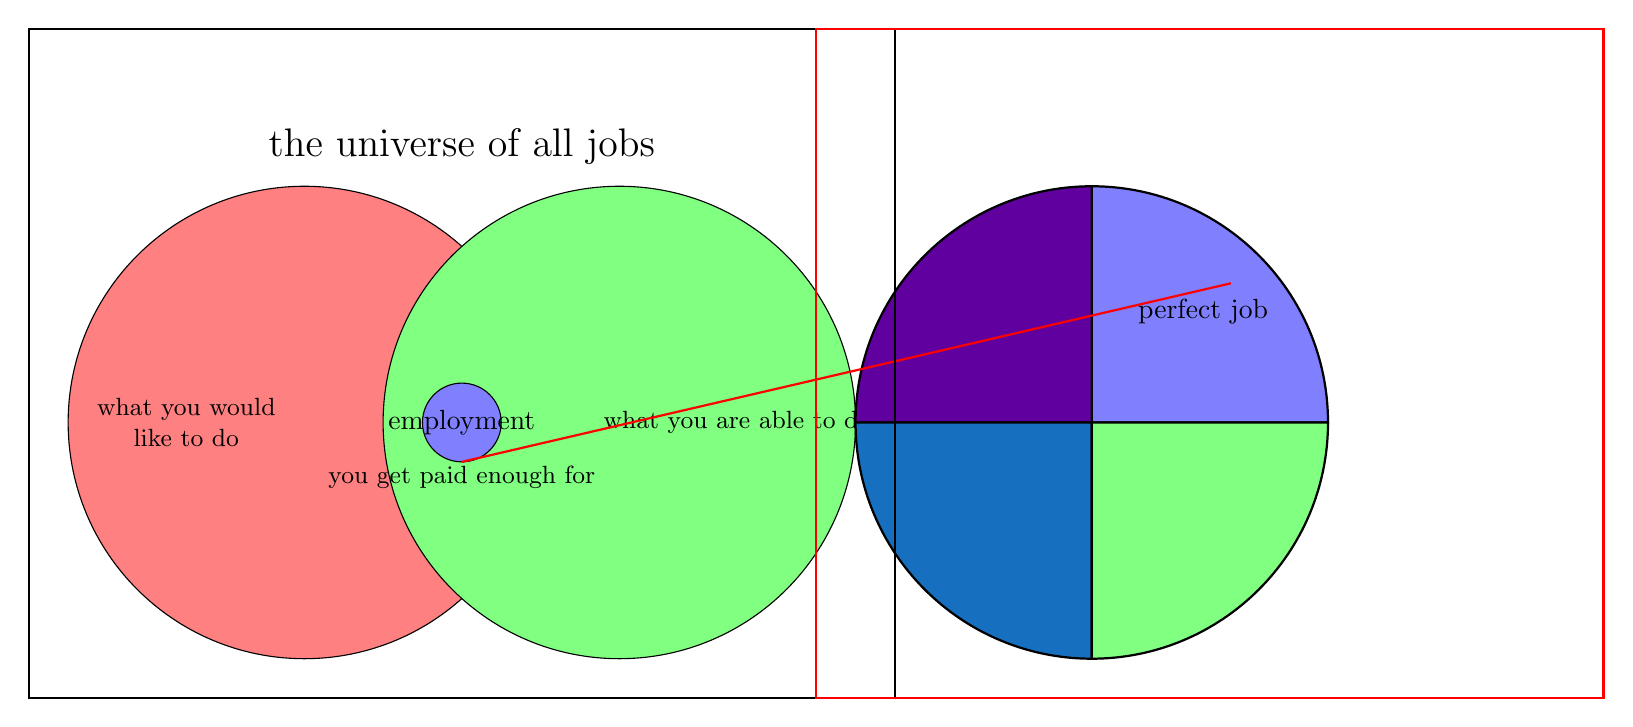
\begin{tikzpicture}[
    title/.style={font=\Large},
    vennlabel/.style={align=center, text width=3.5cm, font=\small},
    piechart/.style={draw=black, thick}
]

% Left Venn Diagram
\draw[fill=red!50!white] (0,0) circle (3cm);
\draw[fill=green!50!white] (4,0) circle (3cm);
% Intersection area
\draw[fill=blue!50!white] (2,0) circle (0.5cm);
% Labels
\node[vennlabel] at (-1.5,0) {what you would like to do};
\node[vennlabel] at (5.5,0) {what you are able to do};
\node at (2,0) {employment};
\node[font=\small] at (2,-0.7) {you get paid enough for};
% Title
\node[title] at (2,3.5) {the universe of all jobs};

% Right Pie Chart
\begin{scope}[xshift=10cm]
\draw[piechart, fill=blue!50!white] (0,0) -- (0:3cm) arc(0:90:3cm) -- cycle;
\draw[piechart, fill=purple!50!blue] (0,0) -- (90:3cm) arc(90:180:3cm) -- cycle;
\draw[piechart, fill=cyan!50!blue] (0,0) -- (180:3cm) arc(180:270:3cm) -- cycle;
\draw[piechart, fill=green!50!white] (0,0) -- (270:3cm) arc(270:360:3cm) -- cycle;
% Perfect job label
\node at (45:2cm) {perfect job};
\end{scope}

% Connecting line
\draw[red, thick] (2,-0.5) -- ($(10,0) + (45:2.5cm)$);

% Borders
\draw[black, thick] (-3.5,-3.5) rectangle (7.5,5);
\draw[red, thick] (6.5,-3.5) rectangle (16.5,5);

\end{tikzpicture}
\end{document}